\documentclass[10pt]{beamer}

\usetheme[progressbar=frametitle]{metropolis}
\usepackage{appendixnumberbeamer}
\usepackage[czech]{babel}
\usepackage{booktabs}
\usepackage[scale=2]{ccicons}
\usepackage{subcaption}

\usepackage{pgfplots}
\usepgfplotslibrary{dateplot}

\usepackage{xspace}
\newcommand{\themename}{\textbf{\textsc{metropolis}}\xspace}

\title{Závislost přítomnosti poslanců na počasí}
%\subtitle{A modern beamer theme}
% \date{\today}
\date{LS 2018/2019}
\author{Šimon Schierrech}
\institute{Semestrální práce z předmětu \textbf{MI-ADM}}
% \titlegraphic{\hfill\includegraphics[height=1.5cm]{logo.pdf}}

\begin{document}

\maketitle

\begin{frame}{Obsah}
  \setbeamertemplate{section in toc}[sections numbered]
  \tableofcontents[hideallsubsections]
\end{frame}

\section{Zadání}

\begin{frame}[fragile]{Zadání}

  \begin{itemize}
      \item Zadání od laboratoře OpenDataLab a firmy Profinit.
      \item Potvrdit nebo vyvrátit souvislost mezi přítomností poslanců a počasím.
  \end{itemize}
  
\end{frame}

\section{Příprava dat}

\begin{frame}{Přítomnost poslanců}
	\begin{itemize}
		\item Poslanecká sněmovna neposkytuje žádné API.
		\item Na stránkách dostupné záznamy o hlasování.
		\item Existující projekty neaktuální.
		\item Tvorba vlastního web-scraperu.
	\end{itemize}
\end{frame}

\begin{frame}{Počasí}
    \begin{itemize}
        \item V Praze jsou čtyři profesionální měřící stanice a Klementinum.
        \item ČHMÚ se vydání dat brání.
        \item Ruční kompilace dat z různých zdrojů.
    \end{itemize}
\end{frame}

\section{Analýza dat o poslancích}

\begin{frame}{Chodí vůbec někdo do sněmovny?}

\begin{figure}
    \centering
    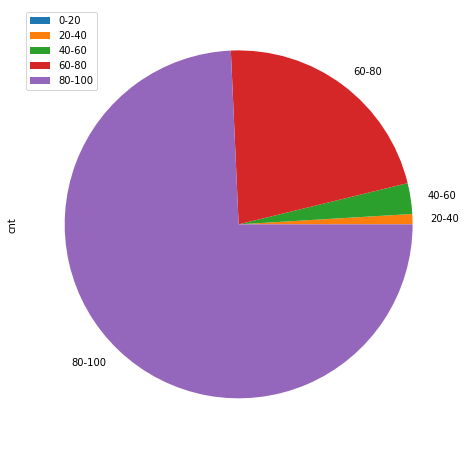
\includegraphics[width=0.55\textwidth]{pie.png}
    \caption{Přehled zastoupení procentuální účasti poslanců na hlasováních}
    \label{fig:presence_pie}
\end{figure}

\end{frame}

\begin{frame}{Kdo jsou ti výtečníci?}
    \begin{columns}
        \begin{column}{0.5\textwidth}
           \begin{tabular}{lr}
                    \hline
                        Jméno & účast (\%) \\
                    \hline
                        Andrej Babiš &  27.36 \\
                      Karel Schwarzenberg &  32.98 \\
                        Martin Stropnický &  41.49 \\
                           Milan Chovanec &  45.98 \\
                         Bohuslav Sobotka &  53.21 \\
                          Antonín Staněk &  56.45
                \end{tabular}
            \end{column}
            \begin{column}{0.5\textwidth}
                \begin{tabular}{lr}
                    \hline
                       Jméno &        účast (\%) \\
                    \hline
                      František Navrkal &  100.00 \\
                           Jiří Hlavatý &  100.00 \\
                           Martin Půta &  100.00 \\
                         Radek Rozvoral &   99.73 \\
                           Lukáš Bartoň &   99.54 \\
                      Miloslav Rozner &   99.54
                \end{tabular}
        \end{column}
    \end{columns}
\end{frame}

\begin{frame}{Přítomnost $\times$ měsíc}
    \begin{figure}
        \centering
        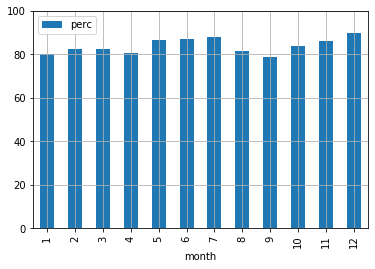
\includegraphics[width=0.7\textwidth]{att_per_month.png}
        \caption{Průměrná přítomnost poslanců v závislosti na měsíci}
        \label{fig:my_label}
    \end{figure}
    
    \emph{Střední hodnota přítomnosti přes všechna hlasování je $84.69$ \%.}
\end{frame}

\section{Klasifikace počasí}

\begin{frame}{Jak poznat hezký den?}
    \begin{itemize}
        \item Velice subjektivní.
        \item Neexistuje žádná metodika.
        \item Vytvořeno více modelů.
    \end{itemize}
\end{frame}

\begin{frame}{Zastoupení \uv{hezkých} dnů v jednotlivých modelech}
    \begin{figure}
\begin{subfigure}{.33\textwidth}
  \centering
  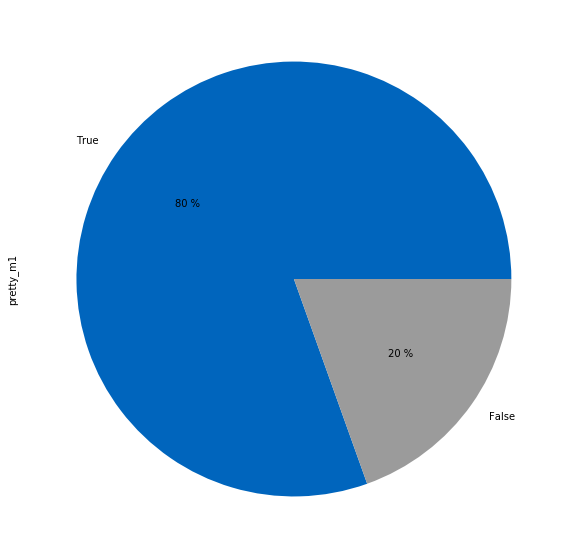
\includegraphics[width=\linewidth]{m1_pie.png}
  \caption{Optimistický model}
  \label{fig:sfig1}
\end{subfigure}%
\begin{subfigure}{.33\textwidth}
  \centering
  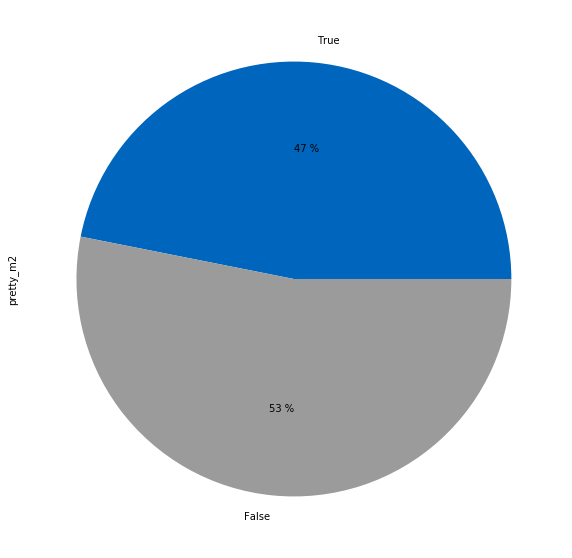
\includegraphics[width=\linewidth]{m2_pie.png}
  \caption{Průměrný model}
  \label{fig:sfig2}
\end{subfigure}
\begin{subfigure}{.33\textwidth}
  \centering
  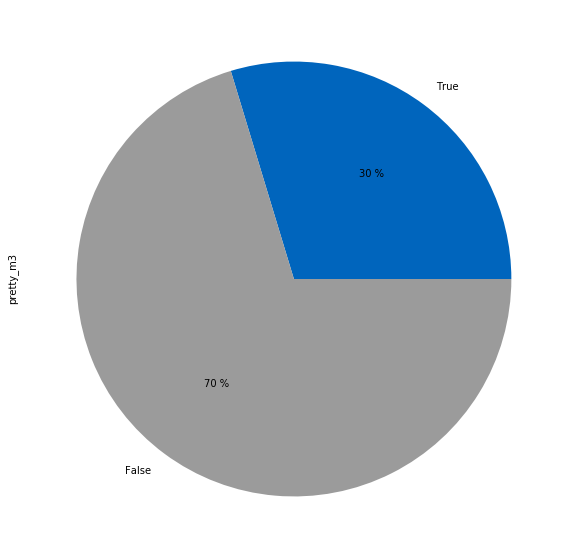
\includegraphics[width=\linewidth]{m3_pie.png}
  \caption{Pesimistický model}
  \label{fig:sfig2}
\end{subfigure}
\caption{Grafy procentuálního zastoupení \uv{hezkých} dnů v jednotlivých modelech}
\label{fig:fig}
\end{figure}
\end{frame}

\section{Vztah přítomnosti a počasí}

\begin{frame}{Závisí přítomnost v PSP na počasí?}
    \begin{figure}
        \centering
        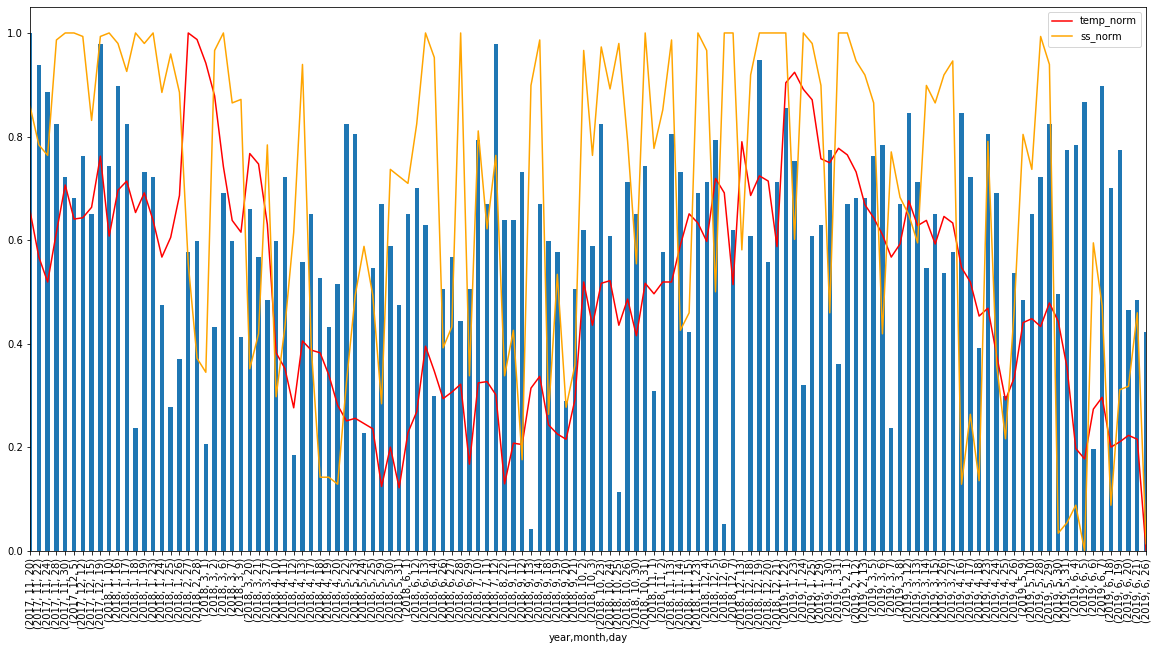
\includegraphics[width=\textwidth]{weather_att.png}
        \caption{Vztah přítomnosti poslanců a různých metrik o počasí}
        \label{fig:my_label}
    \end{figure}
\end{frame}

\begin{frame}{Závisí přítomnost v PSP na počasí?}
    \begin{itemize}
        \item Pro každý z modelů byla metodou \texttt{Point-biserial correlation} vypočtena míra závislosti mezi počtem lidí ve sněmovně a tím, zda je hezký den.
        \item Výsledky ukazují, že vztah mezi veličinami je zanedbatelný.
    \end{itemize}
    
\begin{table}[]
    \centering
    \begin{tabular}{lr}
        \hline 
        \textbf{Model} & \textbf{Korelace} \\
        \hline
        Nadprůměrné teploty & -0.020 \\
        Nadprůměrný svit & 0.020 \\
        Kombinovaný model & 0.077
    \end{tabular}
    \caption{Míra korelace mezi počtem lidí v PSP a hezkým dnem}
    \label{tab:my_label}
\end{table}
\end{frame}

\begin{frame}{Co jednotlivci?}
    \begin{itemize}
        \item Celková účast zjevně s počasím příliš nesouvisí.
        \item Otázka, zda počasí souvisí s přítomností alespoň u jednotlivců, je nasnadě.
        \item Pro každého jednotlivce a každý model vypočítáno metodou. \texttt{Rogers–Tanimoto dissimilarity} míra odlišnosti mezi nepřítomností a hezkými dny.
    \end{itemize}
\end{frame}

\begin{frame}{Co jednotlivci?}
    \begingroup\small
    \begin{columns}
        \begin{column}{0.33\textwidth}
            \centering\begin{tabular}{lr}
                \hline
                Jméno &        Odl. \\
                \hline
                K. Schwarzenberg &  0.55 \\
                M. Stropnický   &  0.58 \\
                A. Babiš        &  0.60 \\
                J. Birke           &  0.63 \\
                A. Staněk      &  0.65 \\
                J. Hamáček         &  0.66 \\
                J. Levová         &  0.68 \\
                M. Chovanec      &  0.68
            \end{tabular}
        \end{column}
        \begin{column}{0.33\textwidth}
            \centering\begin{tabular}{lr}
                \hline
                Jméno &        Odl. \\
                \hline
            D. Ťok           &  0.57 \\
                L. Volný     &  0.57 \\
                S. Juránek &  0.58 \\
                R. Onderka     &  0.58 \\
                V. Filip     &  0.59 \\
                J. Bláha        &  0.59 \\
                M. Bojko      &  0.59 \\
                J. Hamáček       &  0.59 
            \end{tabular}
        \end{column}
        
        \begin{column}{0.33\textwidth}
            \centering\begin{tabular}{lr}
                \hline
                Jméno &        Odl. \\
                \hline
                M. Peksa      &  0.44 \\
                L. Černohorský  &  0.44 \\
                S. Juránek  &  0.44 \\
                J. Schiller       &  0.45 \\
                M. Oborná      &  0.45 \\
                P. Pustějovský  &  0.45 \\
                R. Kubíček      &  0.45 \\
                S. Berkovec &  0.45 
            \end{tabular}
        \end{column}
    \end{columns}
    \endgroup
\end{frame}

\begin{frame}{Závěr}
    Dle zjištěných skutečností se zdá, že přítomnost poslanců v poslanecké sněmovně s počasím nijak výrazně nesouvisí.
\end{frame}

{\setbeamercolor{palette primary}{fg=white, bg=mLightBlue}
\begin{frame}[standout]
  Otázky?
\end{frame}
}

\appendix

{\setbeamercolor{palette primary}{fg=white, bg=mDarkBlue}
\begin{frame}[standout]
  Děkuji za pozornost.
\end{frame}
}

\end{document}
